\chapter{Theoretical Background on Music Emotion Recognition}
\label{chap:TheoreticalBackgroundMER}
\pagestyle{plain}
\vspace{0.5cm}
%\mbox{} \\ \\ \indent

This chapter introduces the readers to the main basics about \gls{mir} and \gls{mer}.
\\
\gls{mir} is an interdisciplinary science where the goal is to retrieve relevant information from music. Researchers belonging to this community may have a background in musicology, psychoacoustics, psychology, academic music study, signal processing, informatics, machine learning, optical music recognition, computational intelligence or some combination of these.
\\ \indent
\gls{mir} is a small but growing field of research with many real-world applications and is being used by businesses and academics to categorize, manipulate and even create music.
\\
A few application to \gls{mir} can be:
\begin{itemize}
	\item Music recommender systems, several already exist, but few are based upon \gls{mir} techniques, some systems do not use just similarity between subjects but also use audio retrieval to achieve better results in music recommendation as in \href{https://www.pandora.com}{Pandora}\footnote{https://www.pandora.com}. 
	\item Intelligent and adaptive digital audio effects aim at design a system that determine the settings of audio effects based on the audio content.
	\item Music recording analysis as track separation, or also instrument recognition.
	\item Automatic music transcription, the process of converting an audio recording into symbolic, such score or a MIDI file.
	\item Automatic music tagging, as musical genre categorization or extraction of other high level features (the usual task for the yearly \gls{mirex}).
\end{itemize}
A broadly part of \gls{mir} is \gls{mer}, where a useful application can be seen in this thesis.
\\
In this chapter will be presented as first an introduction on \gls{mer}. Due to the fact that this field is based on the emotions, they are explained and related to music. Is then presented the emotion space, where emotions are represented on a plane.
\\
Is also shown the general framework of \gls{mer} algorithms based on categorial or dimensional approaches, the music features extraction and selection, followed by some \gls{ml} process to complete the general problem.
\\
To conclude are mentioned some open issues related with \gls{mer}.

\section{Music Emotion Recognition}
\gls{mer} is an important topic in the field of \gls{mir}. Music is often referred as the language of emotion. People tend to listen different songs when in different emotional states. Therefore, categorizing music according to the type of emotion they express is becoming more and more important for internet music service provider. \gls{mer} aims at modeling human emotion perception of music \cite{yang2011music}.
\\
Automatic \gls{mer} allows users to retrieve and organize their music collections in a fashion that is more content-centric than conventional methods based on metadata.
\\
The main challenge is based on the human perception of emotions, their subjective nature of emotion perception. 
Building such a music emotion recognition system, however, is challenging because of the subjective nature of emotion perception. One needs to deal with issues such as the reliability of ground truth data and the difficulty in evaluating the prediction result, which do not exist in other pattern recognition problems such as face recognition and speech recognition. 
\\ \indent
Music plays an important role in human life, even more in the digital age. Never before such a large collection of music has been created and accessed daily by people. Before with the use of compact audio formats with near CD quality such as MP3 and now on with the various streaming services, have greatly contributed to the tremendous growth of digital music libraries.
\\ \indent
Conventionally, the management of music collections is based on catalog metadata, such as artist name, album name, and song title. As the amount of content continues to explode, this conventional approach may be no longer sufficient. The way that music information is organized and retrieved has to evolve to meet the ever increasing demand for easy and effective information access.
\\ \indent
However, music is a complex acoustic and temporal structure, it is rich in content and expressivity.
\\
When an individual engages with music as a composer, performer or listener, a very board range of mental processes is involved, including \textit{representational} and \textit{evaluative}. The representational process includes the perception of meter, rhythm, tonality, harmony, melody, form, and style, whereas the evaluative process includes the perception of preference, aesthetic experience, mood, and emotion. The term evaluative is used because such processes are typically both valences and subjective. Both the representational and the evaluative processes of music listening can be leveraged to enhance music retrieval.
\\
According to a study of \href{https://www.last.fm/home}{Last.fm}\footnote{https://www.last.fm/home}, emotion tagging is the third most frequent type of tags (first is genre and second geographic area) assigned to music pieces by online users.
\\ Even if emotion-based music retrieval was not yet well explored, a survey conducted in 2004 from \cite{lee2004survey} showed that about 28.2\% of the participants identified emotion as an important criterion in music seeking and organization.
\\
The table \ref{table:browse_music} represent the responses of 427 subjects to the question \textit{"When you search for music or music information, how likely are you to use the following search/browse options?"} \cite{lee2004survey}.
\begin{table}[h!]
	\centering
	\begin{tabular}{|l | c|}
		\hline
		Search/Browse by & Positive rate\\ [0.5ex] 
		\hline\hline Singer/Performer 			&		96.2\%	\\ 
		\hline	Title of work(s) 					& 		91.6\%	\\ 
		\hline	Some words of the lyrics 	& 		74.0\% 	\\
		\hline	Music style/genre 				&		62.7\%	\\
		\hline	Reccomendations 				&		62.2\%	\\
		\hline	Similar artist(s)					&		59.3\%	\\
		\hline	Similar music 					&		54.2\%	\\
		\hline	Associated usage				&		41.9\% 	\\
		\hline	Singing								&		34.8\% 	\\
		\hline	Theme(main subject)			&		33.4\% 	\\
		\hline	Popularity							&		31.0\% 	\\
		\hline	\textbf{Mood/emotional state	}	&		\textbf{28.2\%} 	\\
		\hline	Time period						&		23.8\% 	\\
		\hline	Occasions to use				&		23.6\% 	\\
		\hline	Instrument(s)					&		20.8\% 	\\
		\hline	Place/event where heard	&		20.7\% 	\\
		\hline	Storyline of music				&		17.9\% 	\\
		\hline	Tempo								&		14.2\% 	\\
		\hline	Record label						&		11.7\% 	\\
		\hline	Publisher							&		6.0\% 	\\
		\hline
	\end{tabular}
	\caption{Responses of 427 subjects to the question \textit{"When you search for music or music information, how likely are you to use the following search/browse options?"}}
	\label{table:browse_music}
\end{table}
\\
Into another survey \cite{juslin2004expression}, they present findings from an exploratory questionnaire study featuring 141 music listeners (between 17 and 74 years of age) that offers some novel insights. 
\\
Emotions induced by music are subjective phenomena, there are significant differences between individuals. One of the most exciting but difficult endeavors in research on music is to understand how listeners respond to music. It has often been suggested that a great deal of the attraction of music comes from its “emotional powers”. That is, people tend to value music because it expresses and induces emotions.
The table  \ref{table:motivation_music} tries to resume the motivations to the answer \textit{"Why do we listen to music?"}
\begin{table}[h!]
	\centering
	\begin{tabular}{|l | c|}
		\hline
		Motive & Ratio\\ [0.5ex] 
		\hline\hline "To express, release and influence emotions"	&	47\%	\\ 
		\hline "To relax and settle down"										&	33\%	\\
		\hline "For enjoyment, fun, and pleasure"							&	22\%	\\
		\hline "As company and background sound"						&	16\%	\\
		\hline "Because it makes me feel good"								&	13\%	\\
		\hline "Because it's a basic need, I can't live without it"		&	12\%	\\
		\hline "Because I like, love music"										&	11\%	\\
		\hline "To get energized"													&	9\%	\\
		\hline "To evoke memories"												&	4\%	\\ 
		\hline
	\end{tabular}
	\caption{Responses of 141 subjects to the question \textit{"Why do you listen to music?"}}
	\label{table:motivation_music}
\end{table}
\\ \indent
Some music companies, like  \href{https://www.allmusic.com/moods}{Allmusic.com}\footnote{https://www.allmusic.com/moods}, gives the possibility to search music by emotion labels. With these, the user can retrieve and browse artists or albums by emotion.
\\ \indent
Making computers capable of recognizing the emotion of music also enhances the way humans and computers interact. It is possible to play back music that matches the users mood detected from physiological, prosodic, or facial cues. A cellular phone equipped with automatic \gls{mer} function can then play a song best suited to the emotional state of the user; a smart space (e.g. restaurant, conference room, residence) can play background music best suited the people inside it.

\section{Emotions and music}
There is a relationship between music and emotions, that has been the subject of much discussion and research in many different disciplines, like philosophy, musicology, sociology.
\\
In psychological studies, emotion are often divided into three categories:
\begin{itemize}
	\item \textit{Expressed emotion} that the performer tries to communicate with the listener.
	\item \textit{Perceived emotion} represented by music and perceived by the listener.
	\item \textit{Felt} or \textit{Evoked emotion} induced by music and felt by the listener.
\end{itemize}
\gls{mer} focus on perceived emotions because they are less subjective than felt emotions and are often easier to conceptualize. This because felt emotions depends on personal factors and the situation in which the listener processes the song.
From an engineering point of view, one of the main interests is to develop a computational model of music emotion and to facilitate emotion-based music retrieval and organization.
\\
\gls{mir} community has made many efforts for automatic recognition of the perceived emotion of music, various implementations will be presented further in chapter \ref{chap:StateOfTheArt}.
\\ \indent
One of the aims of this thesis, is trying to link perceived and felt emotions, the former through the analysis of the music, the latter, through biometric signals and understand how are they related.

\section{Emotion space}
Now we will focus on the emotion conceptualization alone, since it's central to have a theoretical background to apply then to \gls{mer}.
\\ \indent
The celebrated paper of Hevner \cite{hevner1935expression} from 1934, studied the relationship between music and emotions though experiments where subjects were asked to report some adjectives that came to their mind as the most representative part of a music played. From this have been proposed a large variety of emotion models, like the one presented and used in this thesis.
\\ \indent
Emotions, in the years, were conceptualized in two main approaches, the \textbf{categorical approach} and the \textbf{dimensional approach}. In the following sections will be presented these two different approaches, along with another one used for dynamic emotion recognition.

\subsection{Categorical approach} \label{categorical_approach}
The first assumption of this emotion conceptualization is that emotions are categorized and categories are distinct from each other. Within this approach, it is necessary to assume that there are a limited number of innate and universal emotion categories such as:
\begin{itemize}
	\item Happiness
	\item Sadness
	\item Anger
	\item Fear
	\item Disgust
	\item Surprise
\end{itemize}
All the other emotions can be derived from these "\textit{basic emotions}".
\\
In psychological studies, different researchers have come up with different sets of basic emotions.
\\
For example, a famous categorical approach to emotion conceptualization is Hevner's adjective checklist. He defined eight clusters positioned in circle as in figure \ref{fig:Hevner_clusters}. Adjectives in the same cluster are nearly identical, neighbor clusters have similar meaning. The opposite position of a given cluster is its opposite in emotional sense.
\begin{figure}[h]
    \centering
    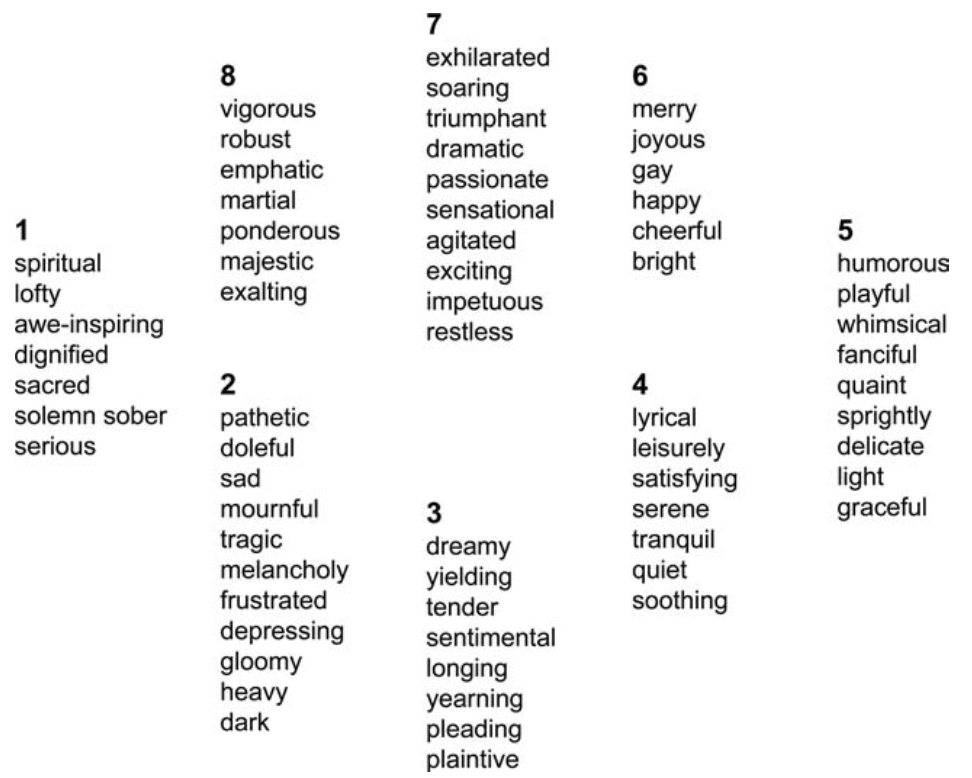
\includegraphics[width=0.8\textwidth]{Hevner_clusters.png} 
	\caption{Eight clusters proposed by Hevner}
    \label{fig:Hevner_clusters}
\end{figure}
\\
Hevner's checklist proposed in 1935 was updated and regrouped into ten groups by Fansworth and into nine groups in 2003 by Schubert.
\\ \indent
Drawback of categorical approach is that the number of primary emotion classes is very small in comparison with the richness of music emotion perceived by humans. The problem is that using a finer granularity it does not necessarily solve the issue because the language for describing emotions is inherently ambiguous and varies from person to person. Using a large number of emotion classes could confuse the subject and is impractical for psychological studies falsing results.

\subsection{Dimensional approach} \label{dimensional_approach}
While categorical approach focuses mainly on the characteristics that distinguish emotions from one another, dimensional approach focuses on identifying emotions based on their position on a small number of emotion "dimensions" called axes, intended to correspond to internal human representation of emotion.
\\ \indent
Several names from researchers gave very similar interpretations of the resulting factors like tension/energy, intensity/softness, tension/relaxation. Most of the factors correspond to the two dimensions of emotion the \textit{valence} (positive and negative affective states) and \textit{arousal} (energy and stimulation level) to create the \gls{va} space. Some studies found that valence as well as intensity, is triggered by the amygdala, while the arousal by the reptilian brain.
\\
Russel, proposed a circumplex model of emotion in \cite{russell1980circumplex} which consist in a two-dimensional, circular structure, as in figure \ref{fig:Russel_va_model} involving the dimensions of valence and arousal. In this structure, emotions that are inversely correlated, are placed across the circle from one another.
\begin{figure}[h]
    \centering
    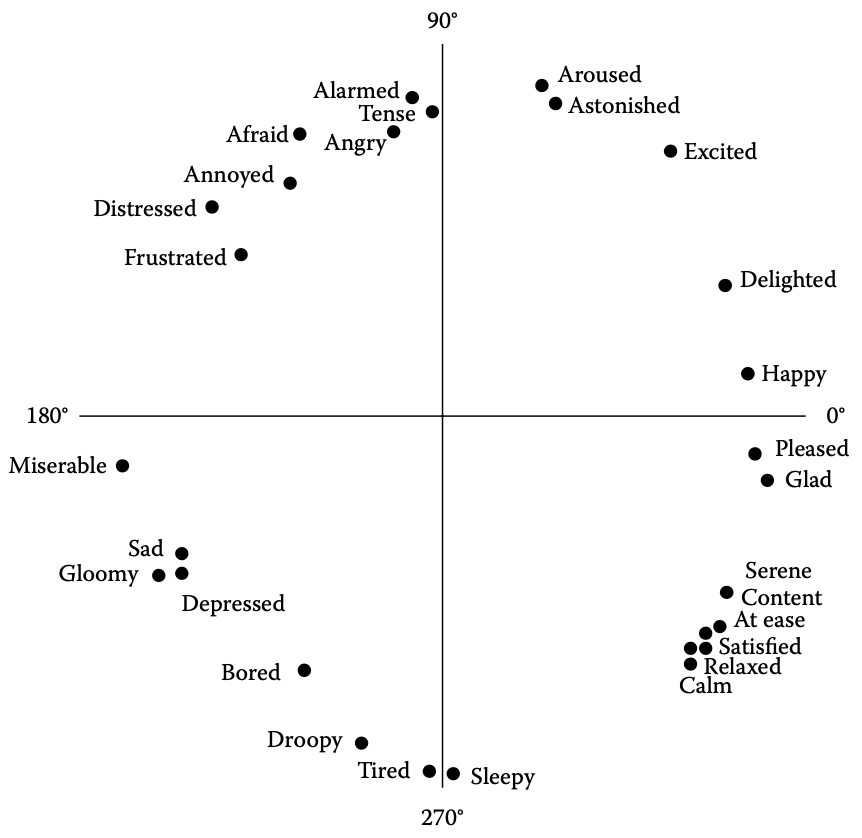
\includegraphics[width=0.7\textwidth]{Russel_va_model.png} 
	\caption{Russel's circumplex model of affect}
    \label{fig:Russel_va_model}
\end{figure}

Emotions that are easy to be confused, such as calm and sadness, appear to have similar valence and arousal values. This result implies that valence and arousal may be the most fundamental and most clearly communicated emotion dimensions among others.
\\
High arousal emotional events are encoded better that non arousing events. Instead of increasing overall attention to an event, an emotionally arousing stimulus decreased attentional resources available for information processing and focused attention only on the arousal-eliciting stimulus.
\\ \indent
The experience of music listening is multidimensional. Different emotions are associated with different music patterns. For example, arousal is associated to:
\begin{itemize}
	\item tempo (fast/slow)
	\item pitch (high/low)
	\item loudness (high/low)
	\item timbre (bright/soft)
\end{itemize}
while valence is associated to:
\begin{itemize}
	\item mode (major/minor)
	\item harmony (consonant/dissonant)
\end{itemize}
as expressed in \cite{gabrielsson2001influence}.
\\
Emotion perception is correlated to the combination of music factor, rarely from just one of them. For example, loud chords and high-pitched chords tends to be feel as more positive valence than soft chords and low-pitched chords.
\\ \indent
Also dimensional approach have some drawbacks. For example, it is argued that dimensional approach blurs important psychological distinctions and consequently obscure important aspects of the emotion process. One example in support of this argumentation is that anger and fear are placed close in the valence-arousal plane but they have very different implications for the organism. Also, it has been argued that using only a few emotion dimension cannot describe all the emotions without residuum.
\\
To overcome this issue, some researchers tired to add a third dimension called \textit{potency}, varying from dominant to submissive, to obtain a more complete picture of emotion. However, this would increase the cognitive load on the subjects and at the same time requires a more complex interface and makes hard to annotate the process. The third dimension problem is still in discussion.

\subsection{Music Emotion Variation Detection}
An important aspect that is not addressed in the previous two paragraphs (\ref{categorical_approach} and \ref{dimensional_approach}) is temporal dynamics. Most researches has focused on music piece that are homogeneous with respect to the emotional plane. However, music can change its emotional expression during the song, becomes important to investigate the time-varying relationship between music and emotion. Here is more useful the dimensional approach to capture the continuous changes of emotional expression as \gls{mevd}. Usually subjects are asked to rate valence and arousal in response of the stimulus over time.
\\
For example, songs can be described by valence and arousal curves as in the following figure:
\begin{figure}[h]
    \centering
    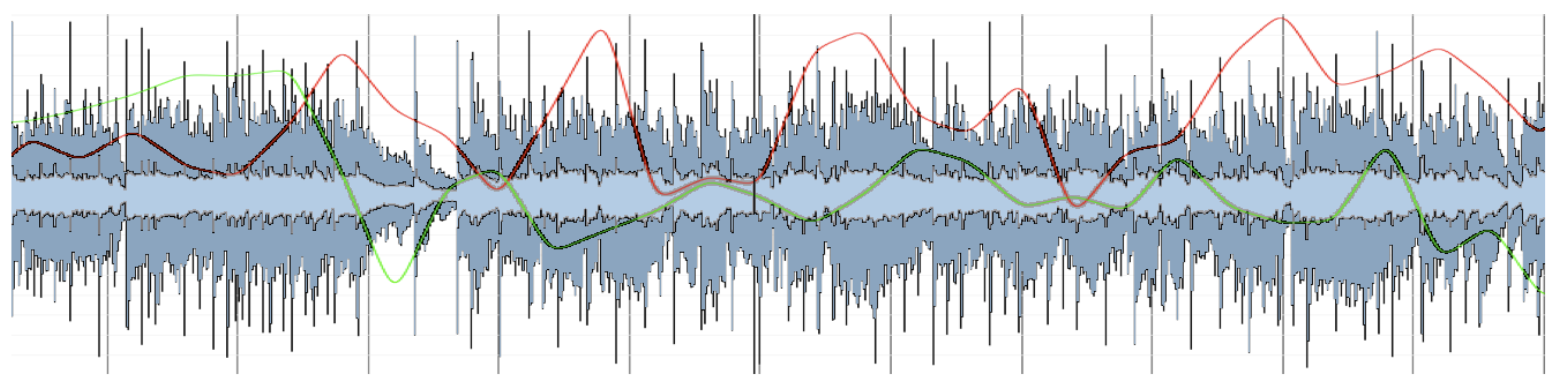
\includegraphics[width=\textwidth]{va_curves.png} 
	\caption{Valence and arousal curves for MEVD}
    \label{fig:va_curves}
\end{figure}

\section{MER algorithms}
\gls{mir} researches have been made to automate \gls{mer} tasks, and the type of music under study has gradually shifted over the past few years from symbolic music to raw audio signal, from Western classical music to popular music. The purpose of \gls{mer} is to facilitate music retrieval and management in the everyday music listening.
\\
In the following section will be presented the general algorithm path for \gls{mer} problems.

\subsection{General framework}
Nowdays, main approaches are still context-based approaches based on human tagging, but it is not possible to annotate a great amount of songs and there is a possibility of human mistakes. To overcome those problems, \gls{ml} and data mining techniques are used to model the relationship between music and emotion. \gls{ml} is used to automatically infer mood and mood variation perceived in songs.
\\
The training and automatic recognition model typically consists of the following steps:
\begin{enumerate}
	\item Data collection: nowadays there are several large-scale dataset covering all sort of music types and genres. Otherwise is desirable to collect data of the different types, getting rid of the effects called "\textit{album effect}" or "\textit{artist effect}" and collect a variety of music pieces. One problem is that there is no consensus on which emotion model or how many emotion categories should be used. Comparing systems that use different emotion categories  and different dataset is impossible. However the issue concerning how many and which emotion classes should be used seem to remain open.
	\item Data preprocessing: to compare music pieces fairly, music pieces are normally converted to a standard format, and since a complete music piece can contain sections with different emotions, $20$ to $30$ second segment is often selected, which is representative of the song (like the chorus part). A good remark of the segment length can be found in \cite{macdorman2007automatic}.
	\item Subjective test: emotion is a subjective matter, so the collection of the ground truth data should be conducted carefully. Annotation methods can be grouped into two categories:
	\begin{itemize}
		\item Expert-based method: which employs a few musical experts to annotate emotions.
		\item Subject-based method: employs a large number of untrained subjects to annotate emotions.
	\end{itemize}
	The ground truth is set by averaging the opinion of all subjects (typically more than 10 subjects per song).
	\\
	It became important to not make a long test, in order to not compromise the reliability of the emotion annotations. Nowadays is introduced the use of listening games.
	\item Collect from human annotators the ground truth emotion labels or emotion values.
	\item Features extraction: a certain number of features are extracted from the music signal to represent the different dimension of music listening like melody, timbre and rhythm.
	\\
	After features extraction, is applied feature normalization, in order to have a standardized visualization.
	\item Apply a learning algorithm between music features and emotion labels/values by training a \gls{ml} model to learn the relationship between emotion and music. Music emotion classification is carried out with classification \gls{ml} algorithms, such as \gls{nn}, \gls{knn}, decision tree, \gls{svm} and \gls{svc}.
	\item Predict emotion of an input song from the resulting computational model.
\end{enumerate}
The music emotion recognition process can be schematized in the figure \ref{fig:MER_process} with a division in training and testing, in order to apply \gls{ml} methods.
\begin{figure}[h]
    \centering
    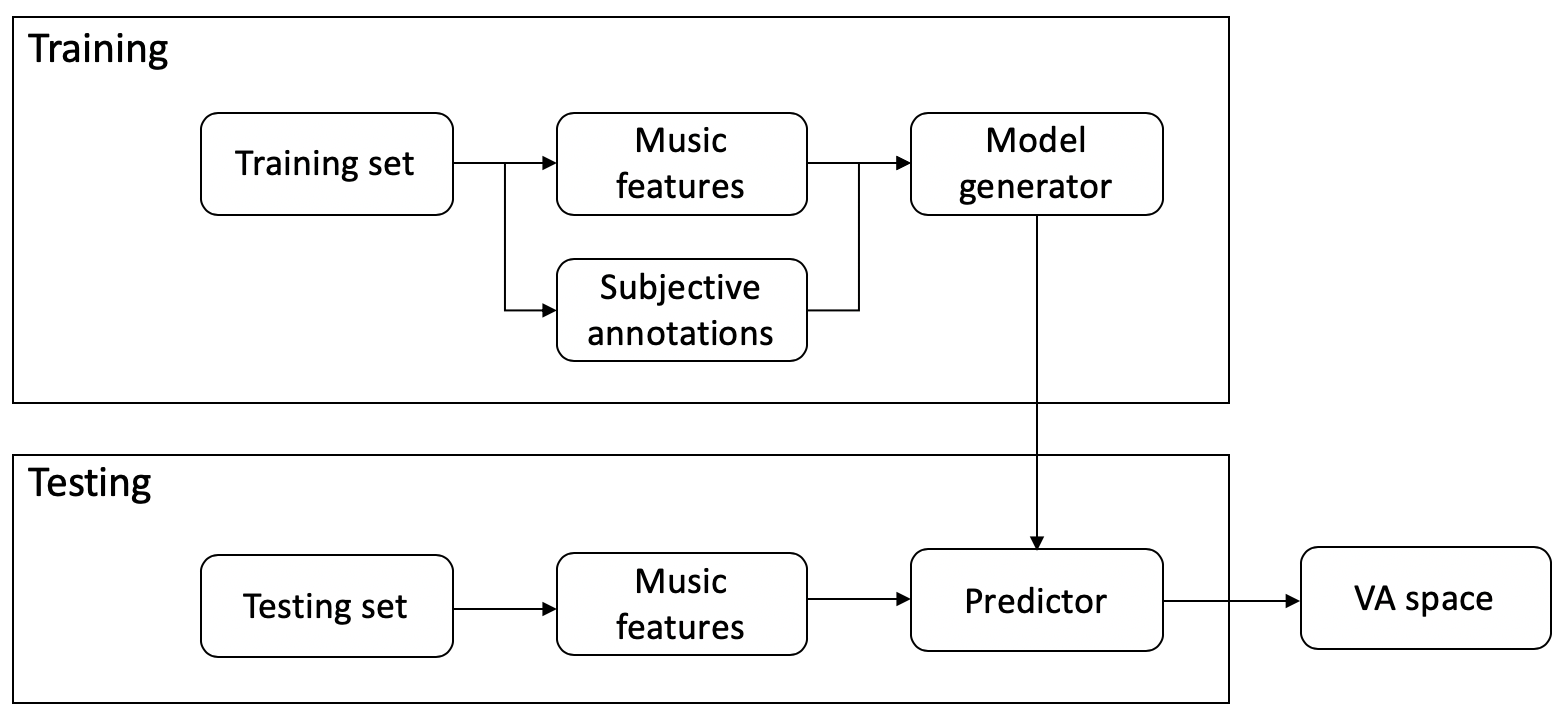
\includegraphics[width=0.9\textwidth]{MER_process.png} 
	\caption{MER general framework process}
    \label{fig:MER_process}
\end{figure}
\\
Researches that work on \gls{mer} can be classified into two approaches, categorical and dimensional, which are based on the emotion representation ideas.
\\
In categorical approach, subjective annotations are global terms, in dimensional approach subjective annotations are point in the \gls{va} space and in \gls{mevd} they are sequences of points in the dimensional space.

\subsection{Categorical approach}
The categorical approach categorizes emotions into a number of discrete classes and applies \gls{ml} techniques to train a classifier. The predicted emotion labels can be incorporated into a text-based or metadata-based music retrieval system.
\\
Advantage of categorical approach is that it is easy to be incorporated into a text-based or metadata-based retrieval system. Emotion labels provide an atomic description of music that allows users to retrieve music through a few keywords.

\subsection{Dimensional approach}
The dimensional approach to \gls{mer} defines emotions as numerical values over \gls{va} plane. A regression model is trained to predict the emotion values that represent the affective content of a song, thereby representing the song as a point in an emotion space. Due to the fact that the emotion plane contain an infinite number of emotion descriptions, the granularity and ambiguity issues are relieved.
\\
\gls{mer} problem became a regression problem, and two independent models, as regressors, are trained to predict separately valence and arousal values.
\\
The dimensional approach requires the subjects to annotate the numerical \gls{va} values. This requirement impose an high cognitive load on the subjects.
\\ \\
Pros and cons of categorical and dimensional approach are schematized in the table \ref{table:pros_cons_categorical_dimensional}.
\begin{table}[h!]
	\centering
	\begin{tabular}{|c|p{0.3\textwidth}|p{0.4\textwidth}|}
	\hline
	& Pros & Cons\\ [0.5ex] 
	\hline\hline Categorical & Intuitive \newline Natural language \newline Atomic description & Lack a unifying model \newline Ambiguous \newline Subjective \newline Difficult to offer fine-grained differentiation \\
	\hline Dimensional & Focus on few dimensions \newline Good user interface & Less intuitive \newline Semantic loss in projection \newline Difficult to obtain ground truth \\
	\hline
	\end{tabular}
	\caption{Pros and cons of categorical and dimensional approaches}
	\label{table:pros_cons_categorical_dimensional}
\end{table}

\section{Music features}\label{music_features}
In MER analysis, an important step is to extract audio features and than apply a feature selection method.
\\
There are several features that can be extracted from audio signal in order to represent five of the most useful perceptual dimensions of music listening:
\begin{itemize}
	\item Energy: dynamic loudness, audio power, total loudness, specific loudness sensation coefficients.
	\item Rhythm: beat histogram, rhythm pattern, rhythm regularity, rhythm clarity, average onset frequency, average tempo.
	\item Temporal: zero-crossing, temporal centroid, log-attack-time.
	\item Spectrum: spectral centroid, spectral rolloff, spectral flux, spectral flatness.
	\item Harmony: salient pitch, chromagram centroid, harmonic change, pitch histogram.
\end{itemize}
These features are just an example of an infinite series of features that can be extracted from audio signals.
\\ \indent
Gabrielsson et al. \cite{gabrielsson2001influence} noted that there are corresponding relations between the dimensional models and music features. Among these features, intensity is a basic feature, which is highly correlated with arousal and is used to predict the arousal dimension \cite{zhang2017feature}.
\\
In \cite{panda2018novel} is shown a table summary of musical characteristics relevant to emotion, reported in \ref{table:musical_features_relevant}.
\begin{table}[h!]
\centering
	\begin{tabular}{|l|l|}
		\hline
		Features & Examples\\ [0.5ex] 
		\hline\hline Timing		&	Tempo, variation, duration, contrast \\ 
		\hline Dynamics			&	Overall level, crescendo/diminuendo, accents \\
		\hline Articulation		&	Overall staccato, legato, variability	 \\
		\hline Timbre				&	Spectral richness, harmonic richness \\
		\hline Pitch				&	High or low \\
		\hline Interval			&	Small or large \\
		\hline Melody			&	Range, direction \\
		\hline Tonality			&	Chromatic-atonal, key-oriented \\
		\hline Rhythm			&	Regular, irregular, smooth, firm, flowing, rough \\ 
		\hline Mode				&	 Major or minor \\ 
		\hline Loudness			&	 High or low \\ 
		\hline Musical form	&	 Complexity, repetition, disruption \\ 
		\hline Vibrato				&	 Extent, range, speed \\ 
		\hline
	\end{tabular}
	\caption{Musical features relevant to MER for \cite{panda2018novel}}
	\label{table:musical_features_relevant}
\end{table}
\\
Despite the identification of these relations, many of them are not fully understood, still requiring further musicological and psychological studies, while others are difficult to extract from audio signals. Nevertheless, several computational audio features have been proposed over the years. While the number of existent audio features is high, many were developed to solve other problems (e.g., \gls{mfcc} for speech recognition) and may not be directly relevant to \gls{mer}.
\\ \indent
Nowadays is not really clear the relationship between low-level and mid-level features and mood. In order to capture different aspects is extracted a large set of features. This create a feature matrix that is then normalized in order to map them on the same range of values.
\\ \indent
After the feature matrix is created is applied a feature selection or feature reduction algorithm to select the best set of features. Feature selection algorithms are based on two different ideas:
\begin{itemize}
	\item \gls{hl} point of view: find the set of features that best model the concept. This lead to the accuracy of machine learning techniques being limited because of the limitation of the hypothesis done.
	\item \gls{ll} point of view: find the set of features that produces the best classification rate.
\end{itemize}

\subsection{Feature selection}\label{feature_selection}
From the machine learning point of view, features are not necessarily of equal importance or quality, and irrelevant or redundant features may lead to inaccurate conclusion. Experiments have shown that, although the performance can thus be improved to a certain extent, using too many features leads to performance degradation \cite{zhang2017feature}.
\\
With an highly discriminant sets of features, is not true that their combination produces a better discriminant power, for example if the set of features is 60, the number of possible combinations are:
\begin{equation}
	n_{combinations} = \sum_{n=1}^{60} \binom{60}{k}
\end{equation}
which is clearly impossible to compute. For this reason is applied some feature selection algorithms.
\\ \indent
An example of feature selection for the categorical approach is the Sequential Feature Selection. It starts from an initial condition, and features are added or removed from a candidate subset while evaluating the \textit{criterion} in two possibilities:
\begin{enumerate}
	\item \gls{sfs}: features are sequentially added to an empty candidate set until the addition of further features does not decrease the criterion.
	\item \gls{sbs}: features are sequentially removed from a full candidate set until the removal of further features increases the chosen criterion.
\end{enumerate}
Another feature selection method is the \gls{mrmr} which select the features with the highest relevance to the target class. Relevance is characterized in terms of \textit{mutual information} which is defined as (given $X$ and $Y$ a pair of random variables):
\begin{equation}
	I(x,y)=\iint p(x,y) \log\dfrac{p(x,y)}{p(x)p(y)} dxdy
\end{equation}
where $p(x,y)$ is the joint probability mass function of $X$ and $Y$, $p(x)$ and $p(y)$ are the marginal probability mass function of $X$ and $Y$ respectively.
\\ \indent
On the other side, for dimensional approach, feature selection is for example RReliefF \cite{robnik2003theoretical}. Basic idea of this algorithm is that try to estimate the quality of each attribute (in this context the features) according to how well their values distinguish between instances that are close each other.
\\
The pseudocode of the RReliefF feature selection algorithm from \cite{robnik2003theoretical}:
\begin{figure}[h]
    \centering
    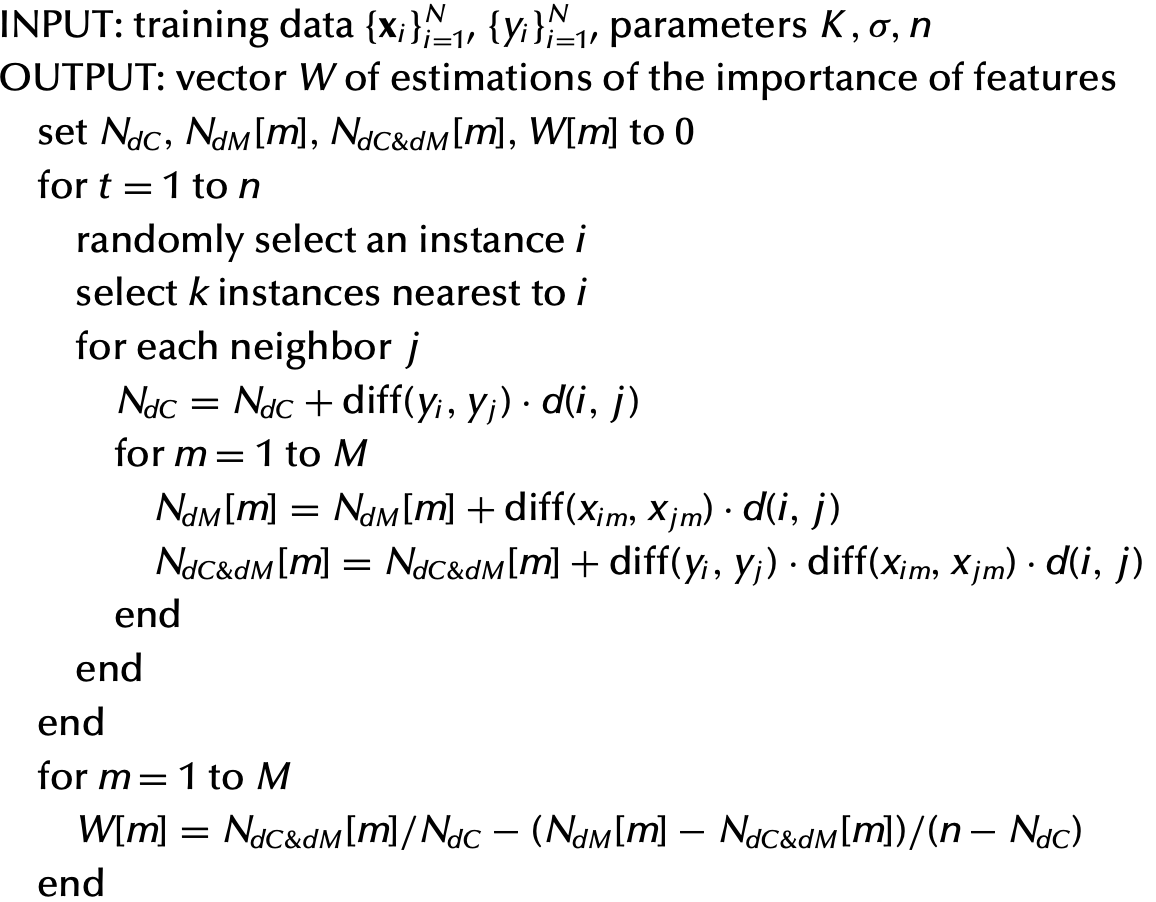
\includegraphics[width=0.8\textwidth]{RreliefF_pseudocode.png} 
	\caption{RReliefF pseudocode}
    \label{fig:RreliefF_pseudocode}
\end{figure}
\\ \indent
Another feature selection for dimensional approach is \gls{pca} and \gls{ica}. The method starts with all features and reduces them one by one, and hence is similar to backward selection. The goal of \gls{ica} is to find a linear representation of non-Gaussian data so that the components are statistically independent, or as independent as possible. While the other well known linear transformation methods (\gls{pca}) benefit from the gaussianity of the data, \gls{ica} improves the classifier performance in the opposite case.

\section{Machine learning}\label{ML}
\gls{ml} is the scientific study of algorithms and statistical models that computer systems use to perform a specific task without using explicit instructions, relying on patterns and inference instead. It is seen as a subset of \gls{ai}. Machine learning algorithms build a mathematical model based on sample data, known as "training data", in order to make predictions or decisions without being explicitly programmed to perform the task.
\\ \indent
\gls{ml} is not just fantasy, it's already here, it has been around for decades in some specialized applications. The first \gls{ml} application that became mainstream was done in 1990s, the \textit{spam filter} \cite{geron2019hands}.
\\
A classical definition came from \textit{Arthur Samuel} in 1959:
\begin{center}
"\textit{Machine Learning is the field of study that gives computers the ability to learn without being explicitly programmed}" 
\end{center}
Another definition, more engineering-oriented is by \textit{Tom Mitchell} in 1997:
\begin{center}
"\textit{A computer program is said to learn form experience E with respect to some task T and some performance measure P, if its performance on T, as measured by P, improves with experience E}"
\end{center}
The main difference between traditional programming and ML is well schematized in the figure \ref{fig:ML_vs_traditional}.
\begin{figure}[h]
    \centering
    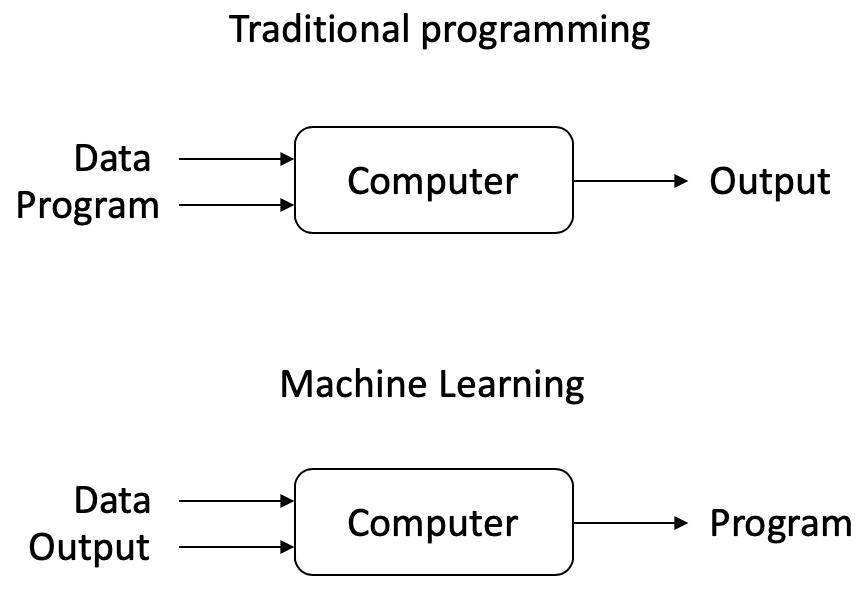
\includegraphics[width=0.6\textwidth]{ML_vs_traditional.png} 
	\caption{Traditional programming versus Machine Learning}
    \label{fig:ML_vs_traditional}
\end{figure}
\\
There are many different \gls{ml} systems. They can be classified in categories based on:
\begin{itemize}
	\item Whether or not they are trained with human supervision (supervised, unsupervised, reinforcement learning).
	\item Whether or not they can learn incrementally on the fly (online and bach learning).
	\item Whether they work by comparing new data points to know data points, or instead detect patterns in the training data and build a predictive model (instance-based and model-based learning).
\end{itemize}
These criteria are not exclusive, they can be combined together.
\\ \indent
In supervised learning, the algorithm builds a mathematical model from a set of data that contains both the inputs and the desired outputs. For example, if the task was determining whether an image contained a certain object, the training data for a supervised learning algorithm would include images with and without that object (the input), and each image would have a label (the output) designating whether it contained the object.
\\
Semi-supervised learning algorithms develop mathematical models from incomplete training data, where a portion of the sample input doesn't have labels.
\\
In unsupervised learning, the algorithm builds a mathematical model from a set of data that contains only inputs and no desired output labels.
\\ \indent
Classification algorithms and regression algorithms are types of supervised learning. Classification algorithms are used when the outputs are restricted to a limited set of values. For a classification algorithm that filters emails, the input would be an incoming email, and the output would be the name of the folder in which to file the email. For an algorithm that identifies spam emails, the output would be the prediction of either "spam" or "not spam", represented by the Boolean values true and false. Regression algorithms are named for their continuous outputs, meaning they may have any value within a range.
\\
In this thesis the focus will be on \textbf{supervised learning}.
\\ \indent
Supervised learning algorithms build a mathematical model of a set of data that contains both the inputs and the desired outputs. The data is known as \textbf{training data}, and consists of a set of training examples. Each training example has one or more inputs and the desired output, also known as a supervisory signal. In the mathematical model, each training example is represented by an array or vector, called \textbf{feature vector}, and the training data is represented by a \textbf{matrix}. Through iterative optimization of an objective function, supervised learning algorithms learn a function that can be used to predict the output associated with new inputs. An optimal function will allow the algorithm to correctly determine the output for inputs that were not a part of the training data. An algorithm that improves the accuracy of its outputs or predictions over time is said to have learned to perform that task.
\\
In order to solve a problem of supervised learning, one has to perform steps:
\begin{enumerate}
	\item Determine the training data type.
	\item Gather a training set.
	\item Determine the input feature representation of the learned function. Here input objects are transformed into feature vector which contains a number of features that describe the object.
	\item Determine the structure of the learned function and corresponding algorithm.
	\item Run the algorithm on the training set and optimize performances on a subset called \textit{validation set} of the training set, or through \textit{cross-validation} (a statistical method used to estimate the accuracy of \gls{ml} models).
	\item Evaluate the accuracy of the model.
\end{enumerate}
There are several algorithms of supervised learning, there are no one that works best on all problems, due to this different algorithms are tested. Most widely used learning algorithms are:
\begin{itemize}
	\item \gls{svm}.
	\item \gls{svr}.
	\item \gls{lr}.
	\item \gls{dt}.
	\item \gls{nn}.
\end{itemize}
Regression and Classification are both problems of supervised machine learning, the main difference between them is that the output variable in regression is numerical (or continuous) while that for classification is categorical (or discrete).
\\ \indent
The task of \gls{mer} is a regression problem both for dimensional, categorical and \gls{mevd}. In dimensional approach, the valence-arousal plane with a continuous space. Each point of the plane is considered an emotion state. This allow to overcome the categorical problem of granularity issue since the emotion plane implicitly offers an infinite number of emotion descriptions.
\\
The regression approach applies a computational model that predicts the valence and arousal values of a music piece, which determine the placement of the music piece in the emotion plane \cite{yang2011music}.
\\ \indent
A user can then retrieve music by specifying a point in the emotion plane according to his/her emotion state, and the system would return the music pieces whose locations are closest to the specified point. Because the 2D emotion plane provides a simple means for user interface, novel emotion-based music organization, browsing, and retrieval can be easily created for mobile devices.

\subsection{Regression approach}
A schematic diagram of the regression approach is in \ref{fig:Regression_scheme} where in the training phase, regression model are trained by learning the relationship between music features $x$ and ground truth emotion values $y$.
\\
\begin{figure}[h]
    \centering
    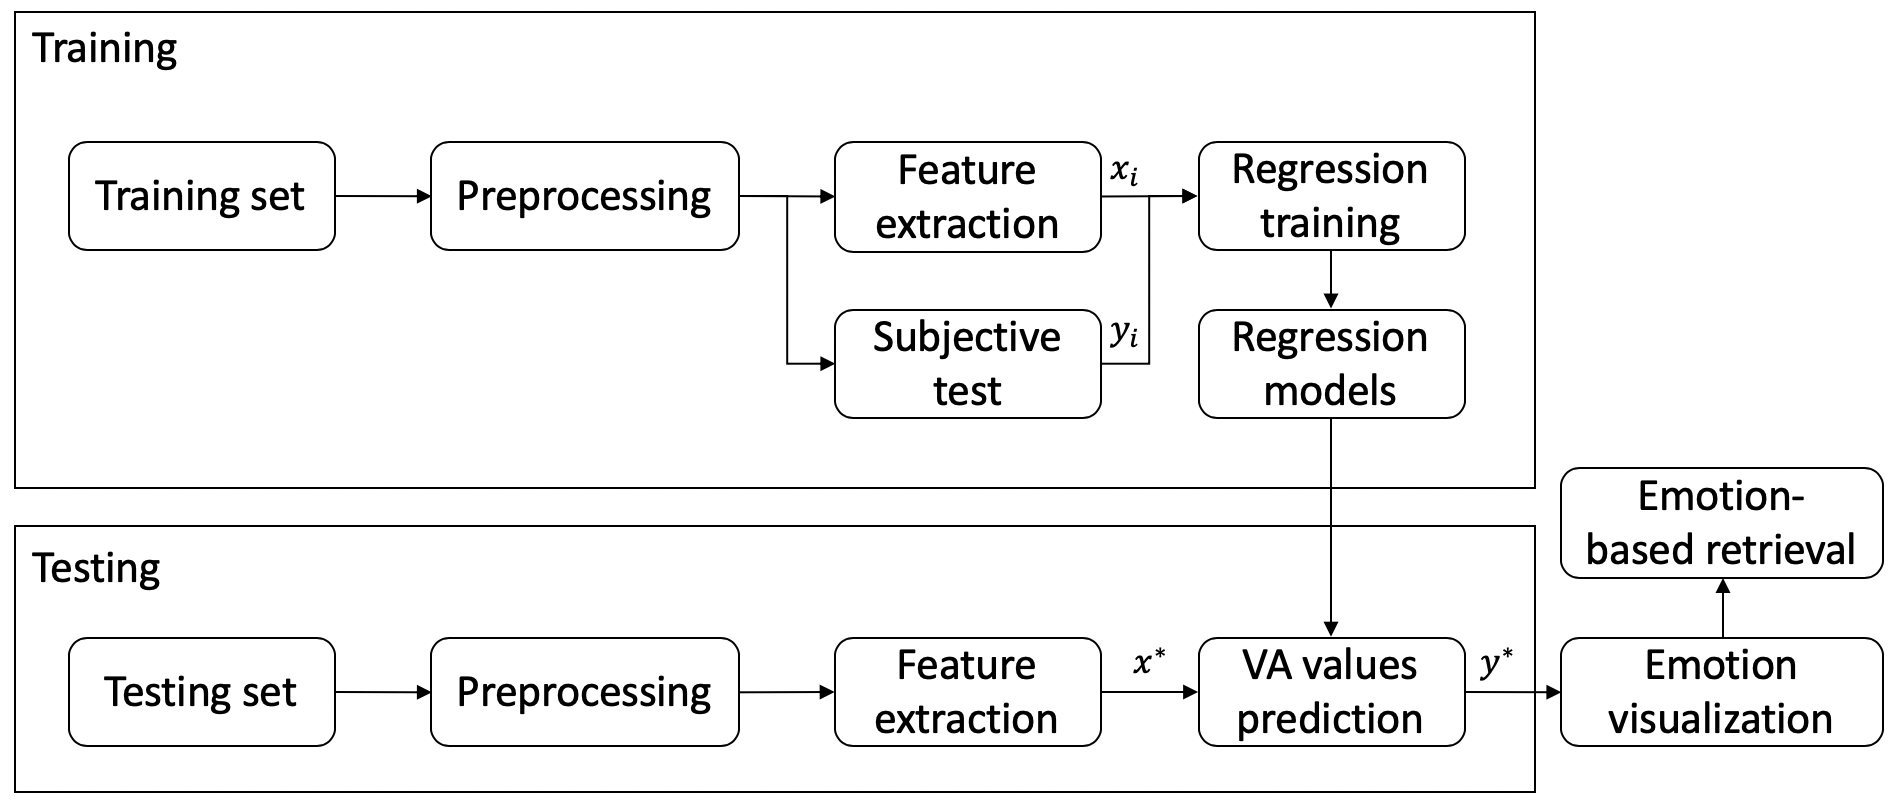
\includegraphics[width=\textwidth]{Regression_scheme.png} 
	\caption{Schematic diagram of a regression approach}
    \label{fig:Regression_scheme}
\end{figure}
\\
Regressors for valence and arousal are denoted with $r_V$ and $r_A$. In the test phase, given the features $x_*$ of an input song, the regressors $r_V$ and $r_A$ can be applied to predict its emotion values:
\begin{equation}
	y_*=[v_*,a_*]^T = [r_V(x_*), r_A(x_*)]^T
\end{equation}
The regression theory aims at predicting a real value from observed variables, in \gls{mer} application music features.  The \gls{va} values are predicted directly from music features and due to this \gls{mer} can be approached as a regression problem.
\\ \indent
Given $N$ inputs $(\textbf{x}_i,y_i)$, with $i \in {1, ..., N}$ where $\textbf{x}_i$ is the feature vector of an object $d_i$ (music piece), and $y_i$ is the real value to be predicted (valence or arousal), a regressor $r(\cdot)$ is created by minimizing the \gls{mse} $\varepsilon$:
\begin{equation}
	\varepsilon = \dfrac{1}{N} \sum_{i=1}^{N} (y_i-r(\textbf{x}_i))^2
\end{equation}
where $r(\textbf{x}_i)$ is the prediction result for $d_i$.
\\
In this thesis in mathematical expressions, \textbf{bold} font is used to represent vectors and matrices.
\\ \indent
To evaluate the performances of the regression approach with various ground truth data spaces, feature spaces and regression algorithms is used the R-squared model, $R^2$ statistics, which is a standard way for measuring the goodness of fit of regression models.
\\
It is calculated as:
\begin{equation}
	R^2(\textbf{y},r(\textbf{X}))=1-\dfrac{N\varepsilon}{\sum_{i=1}^{N} (y_i-\widehat{y})^2}=1-\dfrac{\sum_{i=1}^{N} (y_i-r(\textbf{x}_i))^2}{\sum_{i=1}^{N} (y_i-\widehat{y})^2}
\end{equation}
where $\widehat{y}$ is the mean value of the ground truth. $R^2$ is comparable between experiments thanks to the normalization of the total squared error $N\varepsilon$ by the energy of the ground truth. The value of $R^2$  lies in $[-\inf;1]$ where $R^2=1$ means the model perfectly fits the data, while a negative $R^2$ means the model is even worse than simply taking the sample mean.
\\ \indent
The regression approach to \gls{mer}, however, is not free of issues. First, the regression approach suffers from the subjectivity issue of emotion perception as it assigns the valence and arousal values to a music piece in a deterministic way. It is likely that different users perceive different emotion values in the music piece. Second, the regression approach requires numerical emotion ground truth to train the computational model, but performing such an emotion rating is a heavy cognitive load to the subjects.

\section{Open issues of Music Emotion Recognition} \label{issues}
As \gls{mer}  is a quite new domain, there are some elements that have no clear answer. Four of these issues are:
\begin{enumerate}
	\item Ambiguity and Granularity of emotion description: issue related to the relationship between emotions and the affective terms that denote emotions and the problem of choosing which and how many affective terms to be included in the taxonomy. Emotions are fuzzy concepts, there are main synonyms and similarities between different terms. In general, classification accuracy of an automatic model is inversely proportional to the number of classes considered \cite{van2006emotion}.
	\item Heavy cognitive load of emotion annotation: to collect data for training an automatic model, is typically conducted a subjective test by inviting human subjects to annotate the emotion of music pieces. The problem is that, to reduce the management effort, each music piece is annotated by two or three musical \textit{experts} to gain consensus of the annotation result. Everyday contexts, in which musical experts experience is so different from those non-experts, require separate treatment. Since \gls{mer} system is expected to be used in the everyday context, the emotion annotation should be carried out by \textit{ordinary people}.
	\item Subjectivity of emotional perception: music perception is intrinsically subjective and is under the influence of many factors, such as cultural background, age, gender, personality and so forth. Therefore conventional categorical approaches that simply assign one emotion class to each music piece in a deterministic manner do not perform very well in practice.
	\item Semantic gap between \gls{ll} audio signal and \gls{hl} Human perception: it is difficult to accurately compute emotion values, and what intrinsic element of music causes a listener to create a specific emotional perception is still far from well understood.
\end{enumerate}
